\chapter{Execução do Estudo Observacional}
\label{ch:execucao}

Este capítulo apresenta os processos, etapas e ferramentas utilizados para a realização do estudo nesta pesquisa. Serão tratados detalhes sobre preparação dos artefatos, no caso as histórias de usuário, a adaptação da extensão Cypress Copilot e o ambiente de execução do caso CAPJu.

\section{Preparação dos Artefatos}
\label{sec:preparacao-artefatos}

As histórias de usuário do CAPJu feitas durante o semestre 2023/1 estavam disponíveis no ZenHub\footnote{Disponível em: \url{https://app.zenhub.com/workspaces/2023-1-capju-64320b44af1e32d8b7b66b3f/board}.}, então utilizamos as tags US e frontend, pois a pesquisa trata de identificação de elementos de interface e testes de sistema, e sobraram 26 histórias de usuário de 58. Os critérios de escolha para as histórias de usuário foram ter pelo menos um critério de aceitação, ter sido feita durante o semestre 2023/1, estar fechada e não ser repetida. Também ficou acordado que cada critério de aceitação seria utilizado para a escrita de um cenário BDD; dessa forma, uma história de usuário com três critérios de aceitação se transformaria em três cenários BDD. Após aplicar esses critérios, sobraram 23. A Figura \ref{fig:us06} apresenta um exemplo de história de usuário.

\begin{figure}[htbp]
    \caption{Exemplo de história de usuário do CAPJu (US06 -- Status do processo)}
    \centering
    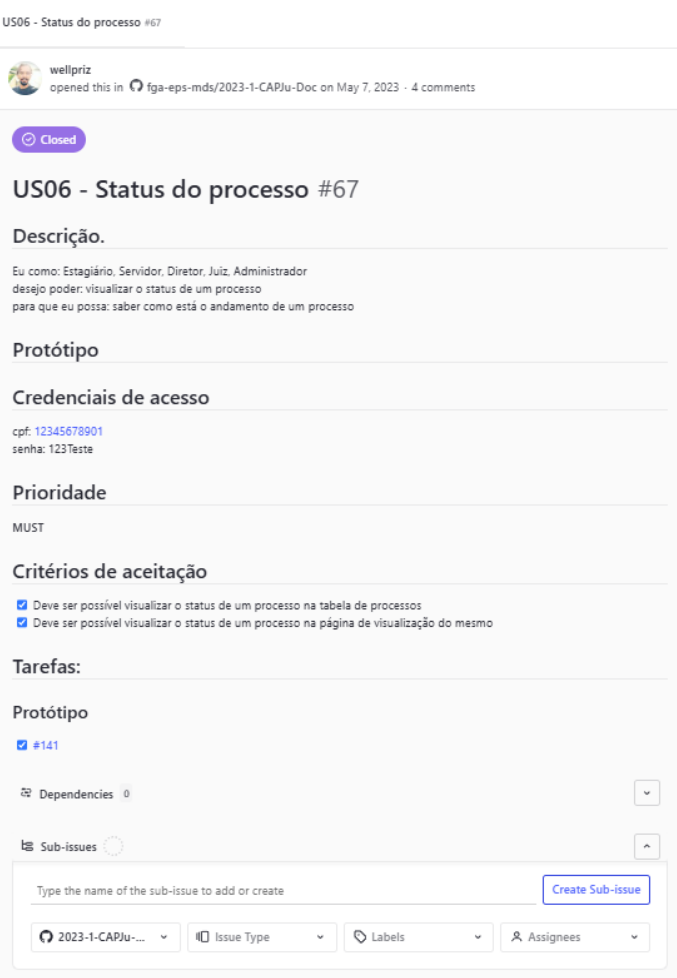
\includegraphics[width=0.6\linewidth]{figuras/US06.png}
    \caption*{Fonte: ZenHub do projeto CAPJu (2023)}
    \label{fig:us06}
\end{figure}

As 23 histórias de usuário somaram 37 critérios de aceitação, mas apenas 27 critérios de aceitação foram transformados em cenários BDD. Os 10 critérios de aceitação que sobraram não foram transformados em cenários BDD, pois a história de usuário 7 não tinha sido implementada; as 28, 37 e 39 possuíam bugs; a 19 não dizia exatamente o que deveria ser testado; e três critérios de aceitação da 1 não foram transformados em cenários por não especificarem com precisão o que testar. Os cenários foram escritos em Gherkin, no formato Given-When-Then, e em inglês, idioma em que a extensão Cypress Copilot foi avaliada por \citeonline{Nettur2025}. Todos os cenários BDD foram escritos por nós, os autores da pesquisa. Para a identificação dos elementos de interface, os seletores foram passados dentro dos cenários BDD. No total, 18 das 23 histórias de usuário tiveram pelo menos um cenário com código gerado. Os 27 cenários podem ser acessados na Tabela 4\footnote{Disponível em: \url{https://docs.google.com/spreadsheets/d/1rJ2EbBNmPHfG4oifdnGyCCSfjqGXW0kYhDEKt6rSJ24/edit?usp=sharing}.}.

\section{Adaptação do Cypress Copilot}
\label{sec:adaptacao-cypress-copilot}

O artigo ``Cypress Copilot: Development of an AI Assistant for Boosting Productivity and Transforming Web Application Testing'', de \citeonline{Nettur2025}, descrito na Seção \ref{sec:rsl-ferramentas}, desenvolveu uma extensão para o VS Code chamada Cypress Copilot, na qual é possível utilizar modelos da OpenAI para gerar código Cypress dividido em duas partes, no caso, Page Object Class Code e Step Definition Code, a partir de cenários BDD. Essa solução se aproxima muito do que queremos em nossa questão de pesquisa, que é ``De que maneira as especificações BDD devem ser escritas e detalhadas para que sistemas baseados em IA consigam identificar os elementos de interface gráfica necessários para criar testes automatizados em nível de sistema?''. Então, fizemos um fork no GitHub\footnote{Disponível em: \url{https://github.com/gustavofbs/Cypress-Copilot}.} para adaptar essa ferramenta para ser útil em nossa pesquisa.

A primeira mudança foi possibilitar que a extensão pudesse reconhecer os identificadores de elementos e os textos, e identificar um elemento específico dentre elementos repetidos com o mesmo identificador. Isso foi feito porque queríamos que o código gerado tivesse exatamente os identificadores de elementos necessários para que ele rodasse no Cypress na aplicação original, no caso, o CAPJu. No artigo do Cypress Copilot, a extensão foi validada com cerca de 55 histórias de usuário coletadas de fontes públicas e em três sites de demonstração, fora de ambientes de produção, e não em um projeto real de desenvolvimento \cite{Nettur2025}. A solução adotada foi escrever o seletor diretamente no cenário, entre parênteses, no próprio passo, como em \Verb[breaklines,breakanywhere]|fills in the CPF field(input[name="cpf"])|. Também foram utilizados outros artifícios, como o índice \Verb[breaklines,breakanywhere]|[N]|, que indica qual elemento, entre vários com o mesmo seletor, deve ser usado, e o \Verb[breaklines,breakanywhere]|[text: ...]|, que indica o texto a ser validado. No fluxo original da ferramenta, o usuário tem que inserir manualmente os identificadores dos elementos no código gerado \cite{Nettur2025}. Como o seletor é escrito dentro do próprio cenário, a IA o utiliza, mas não o detecta na interface. A Figura \ref{fig:bdd-identificadores} apresenta um exemplo de BDD com identificadores.

\begin{figure}[H]
    \caption{Exemplo de cenário BDD com identificadores de elementos}
    \centering
    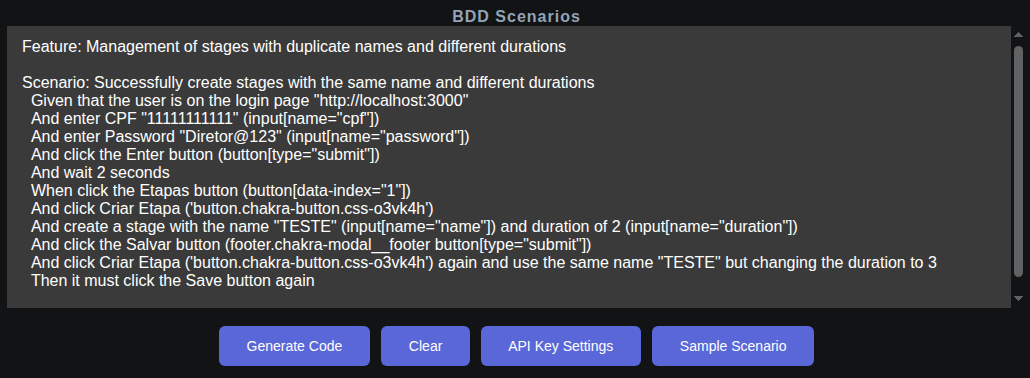
\includegraphics[width=1\linewidth]{figuras/bdd_exemplo_cenario.png}
    \caption*{Fonte: Autores (2026).}
    \label{fig:bdd-identificadores}
\end{figure}

A segunda mudança complementou a primeira por meio das Regras 0, 1, 13, 15 e 16, que envolveram a reescrita do system prompt que é uma mensagem enviada ao modelo antes da geração do código e diz a ele quais regras deve seguir e o que deve fazer. O system prompt foi reescrito com um conjunto de regras que definem como o modelo deve interpretar o BDD e gerar o código. O modelo utilizado foi o GPT-4o, que teve o melhor desempenho entre os avaliados por \citeonline{Nettur2025} quando combinado ao few-shot chain. Utilizamos regras explícitas passadas no system prompt, diferentemente do few-shot adotado no artigo.

A terceira mudança foi possibilitar que a extensão conseguisse calcular as oito métricas de completude (1.1 a 1.8) para steps e POM de cada código gerado e também as exibisse na interface da extensão, dentro do VS Code, após gerar o código. A métrica 1.9 é obtida por meio da execução do código gerado no Cypress (Seção \ref{sec:ambiente-execucao}), pois, se a sintaxe tiver problemas, o código não roda no Cypress e dá erro.

\subsection{Coleta dos Seletores}
\label{sec:coleta-seletores}

Para que a extensão conseguisse gerar um código de teste automatizado que realmente rodasse no Cypress, ela teria que ter os identificadores de elementos corretos. O projeto CAPJu foi rodado localmente e aberto no navegador Chrome e, dessa forma, conseguimos pegar os elementos usando a ferramenta de seleção de elementos do DevTools e a opção ``Copiar seletor'' (Copy selector), com o clique do botão direito sobre o elemento destacado no HTML. Essa foi uma das formas mais utilizadas para pegar os seletores CSS. Em alguns casos, porém, o seletor copiado pelo DevTools não funcionava nos testes, e o elemento também não possuía um id que pudesse ser utilizado. Nessas situações, o seletor foi construído manualmente a partir da estrutura do HTML.

O critério que usávamos para considerar um seletor estável era gerar o código na extensão e ir testando se o Cypress conseguia usar o elemento que queríamos por meio daquele seletor e se ele não mudava a cada execução, o que era importante. Essa validação foi feita manualmente, por tentativa e erro, e não por um procedimento automatizado.

\subsection{Refinamento do System Prompt Code}
\label{sec:refinamento-system-prompt}

O system prompt não foi escrito de uma vez, ele passou por sucessivos refinamentos até chegar a uma versão final. Uma segunda IA, no caso o Claude, foi utilizada para que as regras fossem escritas de uma forma que outra IA entendesse. Esses refinamentos foram registrados em três tabelas, que serviram para calibrar o system prompt. Uma quarta tabela registra a execução definitiva, já com o system prompt final. As tabelas têm as seguintes colunas:

\begin{itemize}
    \item \textbf{US}: identificação da História de Usuário à qual o critério de aceite pertence;
    \item \textbf{BDD Scenario}: o cenário no formato Given-When-Then que descreve o critério de aceite a ser testado;
    \item \textbf{Page Object Class Code}: o código da classe de Page Object gerado a partir do BDD scenario;
    \item \textbf{Step Definition Code}: o código dos Step Definitions gerado a partir do BDD scenario;
    \item \textbf{Feature}: o arquivo .feature correspondente ao cenário, no padrão Gherkin;
    \item \textbf{System Prompt Code}: o system prompt utilizado naquela tentativa/versão para orientar a geração do código;
    \item \textbf{T.M Gerados - Step Definitions / POM}: quantidade total de métodos gerados em cada artefato (1.1 e 1.3);
    \item \textbf{Métodos com/sem Implementação - Step Definition / POM}: quantos desses métodos vieram com implementação completa, e quantos ficaram vazios/pendentes;
    \item \textbf{Fração com/sem Implementação - Step Definition / POM}: a mesma contagem anterior, expressa em proporção sobre o total gerado;
    \item \textbf{Iterações}: número de tentativas/rodadas necessárias até se obter um resultado satisfatório (ou até o encerramento da análise daquele item);
    \item \textbf{Observações}: anotações livres sobre particularidades, dificuldades ou pontos de atenção identificados durante a execução daquele cenário.
\end{itemize}

A coluna Iterações conta as rodadas de geração e ajuste feitas em cada cenário, e na Tabela 4 existe uma coluna a mais, chamada Execution, que registra se o código gerado rodou no Cypress completamente ou não, por meio de S (rodou) e N (não rodou). Essas tabelas registram a execução dos cenários BDD referentes às histórias de usuário e suas métricas. A primeira tabela serviu como exploração para entender a interface e criar regras no system prompt, de forma que o Cypress Copilot conseguisse gerar um código Cypress para aquele cenário. Então, ela não possui padronização, pois o system prompt registrado para cada cenário tinha o objetivo de fazer aquele cenário específico passar.

A segunda tabela foi a primeira tentativa de escrita de um system prompt único que funcionasse para todos os cenários, aproveitando as regras criadas na exploração da Tabela 1. Porém, ainda teve problemas, como, por exemplo, na história de usuário 18, em que o código gerado resumia o texto que deveria ser validado na tela e não o usava literalmente, causando erros.

A terceira tabela ajustou os cenários BDD e resolveu os problemas anteriores por meio de um system prompt padronizado, que conseguiu gerar código de teste Cypress para os 27 cenários escritos. Os outros 10 critérios de aceite não tiveram cenário, pelos motivos descritos na Seção \ref{sec:preparacao-artefatos}. Todas essas tabelas estão registradas em uma planilha\footnote{Disponível em: \url{https://docs.google.com/spreadsheets/d/1rJ2EbBNmPHfG4oifdnGyCCSfjqGXW0kYhDEKt6rSJ24/edit?usp=sharing}.}. O system prompt das Tabelas 3 e 4 é idêntico e foi congelado após a Tabela 3, e só o cenário BDD varia entre uma tentativa e outra. Com um system prompt padronizado, podemos nos focar nos cenários BDD, validando se a extensão modificada consegue gerar código de teste automatizado Cypress a partir do BDD. O system prompt final está disponível no Apêndice \ref{ap:system-prompt}.

\subsection{Regras do System Prompt Code}
\label{sec:regras-system-prompt}

Durante a criação do system prompt com o objetivo de obter um system prompt padronizado, para que pudéssemos focar só nos cenários BDD, foram escritas várias regras para que o modelo de IA entendesse o que deveria fazer e como interpretar o BDD para escrever o código de teste Cypress. Abaixo serão listadas todas as regras e por que elas existem.

\textbf{Regra 0 -- Nunca inventar seletores.} Quando o BDD traz um seletor explícito, entre parênteses ou em \Verb[breaklines,breakanywhere]|[text: ...]|, ele deve ser usado literalmente em \Verb[breaklines,breakanywhere]|cy.get()|, sem ser trocado por \Verb[breaklines,breakanywhere]|cy.contains()| nem por um seletor ``adivinhado''. O erro mais crítico na geração de testes com IA é o modelo criar um seletor plausível, baseado no nome do elemento, em vez de usar o real, o que faz o teste falhar na interface mesmo com código correto.

\textbf{Regra 1 -- O seletor vira comentário.} O seletor, o índice ou o texto de asserção sai da string do passo, que fica só com texto e \Verb[breaklines,breakanywhere]|{string}|, e é preservado no código como comentário \Verb[breaklines,breakanywhere]|// bdd:|. A geração do Page Object só recebe o arquivo de steps e, como o código é gerado em duas chamadas (Regra 17), sem o comentário o seletor se perderia entre elas.

\textbf{Regra 2 -- Botões por texto.} Quando o BDD não traz seletor explícito, o botão é localizado por \Verb[breaklines,breakanywhere]|cy.contains('button', 'texto')|. A regra complementa a Regra 0, dando ao modelo uma opção válida para os casos sem seletor, para que ele não tente inventar um.

\textbf{Regra 3 -- Botões de aba.} Elementos de aba usam \Verb[breaklines,breakanywhere]|cy.contains('button[role="tab"]', 'texto')| em vez de \Verb[breaklines,breakanywhere]|cy.contains('button', 'texto')|, porque, em interfaces com abas, o seletor genérico pode capturar um botão errado, com texto parecido em outro ponto da tela.

\textbf{Regra 4 -- Apenas Given/When/Then.} And e But são proibidos, e cada And é mapeado para o bloco anterior (Given, When ou Then). A biblioteca \Verb[breaklines,breakanywhere]|@badeball/cypress-cucumber-preprocessor| não exporta And e But, e o código gerado quebraria por erro de importação.

\textbf{Regra 5 -- Imports relativos.} Os imports usam caminhos relativos (\Verb[breaklines,breakanywhere]|'../pages/LoginPage'|) e não aliases (\Verb[breaklines,breakanywhere]|@pages/LoginPage|), pois o projeto não tem aliases configurados e usá-los causaria erro de módulo não encontrado na hora de rodar o teste.

\textbf{Regra 6 -- Nome do arquivo igual ao nome da classe.} A classe declarada e o arquivo importado devem ter o mesmo nome (a classe \Verb[breaklines,breakanywhere]|AdicionarObservacaoPage| fica no arquivo \Verb[breaklines,breakanywhere]|AdicionarObservacaoPage.js|). Isso evita erro de importação.

\textbf{Regra 7 -- Classe estática com exportação nomeada.} O Page Object segue o padrão \Verb[breaklines,breakanywhere]|export class ClassName { static method() {...} }|, importado como \Verb[breaklines,breakanywhere]|import { ClassName } from '../pages/ClassName'| e chamado como \Verb[breaklines,breakanywhere]|ClassName.method()|. A regra padroniza a arquitetura do código gerado, para que todos os Page Objects sigam a mesma convenção e sejam mais fáceis de manter e revisar.

\textbf{Regra 8 -- Timeout apenas em \texttt{cy.get()}.} A opção \Verb[breaklines,breakanywhere]|{ timeout: N }| fica somente em \Verb[breaklines,breakanywhere]|cy.get()|, pois em \Verb[breaklines,breakanywhere]|.click()| ou \Verb[breaklines,breakanywhere]|.should()| ela não tem o efeito esperado e pode causar falhas silenciosas no teste.

\textbf{Regra 9 -- Intercept antes da ação.} O comando \Verb[breaklines,breakanywhere]|cy.intercept()| deve vir antes da ação que dispara a requisição de rede, porque, se for configurado depois, a requisição já pode ter sido feita e o intercept não captura nada.

\textbf{Regra 10 -- Esperas explícitas isoladas.} O \Verb[breaklines,breakanywhere]|cy.wait(N)| fica em seu próprio método ou linha, sem se misturar com outra lógica. Assim, se mantém a rastreabilidade entre o passo ``aguarda N milissegundos'' do BDD e o código gerado, evitando que a espera fique escondida em um método com outro propósito.

\textbf{Regra 11 -- Asserções.} A regra define o comando de cada tipo de verificação (conteúdo de texto ou visibilidade) e proíbe encadear \Verb[breaklines,breakanywhere]|.contains()| antes de \Verb[breaklines,breakanywhere]|.should('be.visible')|, pois isso muda o ``sujeito'' da asserção seguinte e o teste passa a verificar a coisa errada.

\textbf{Regra 12 -- Tudo passa pelo Page Object.} Os Step Definitions não podem ter comandos Cypress diretos (exceto \Verb[breaklines,breakanywhere]|cy.visit()| e \Verb[breaklines,breakanywhere]|cy.wait()|), e toda interação passa por um método do Page Object. É a regra que garante a adoção do padrão Page Object Model, pois obriga a existir um método do Page Object para cada interação.

\textbf{Regra 13 -- Seletores repetidos viram \texttt{.eq(N)}.} Elementos que compartilham o mesmo seletor ao longo dos passos são numerados com um contador crescente: a primeira ocorrência usa \Verb[breaklines,breakanywhere]|.eq(0)|, a segunda \Verb[breaklines,breakanywhere]|.eq(1)|, e assim por diante. Sem indexação, \Verb[breaklines,breakanywhere]|cy.get()| pegaria sempre o primeiro elemento encontrado, ignorando qual instância o BDD queria.

\textbf{Regra 14 -- Texto literal, a menos que esteja entre aspas.} Texto entre aspas no BDD vira o placeholder \Verb[breaklines,breakanywhere]|{string}|, e texto sem aspas permanece fixo no passo. Se todo texto virasse \Verb[breaklines,breakanywhere]|{string}|, o passo perderia precisão e não distinguiria um valor variável de um texto fixo esperado.

\textbf{Regra 15 -- \texttt{[text: ...]} é cópia fiel.} O texto entre \Verb[breaklines,breakanywhere]|[text:| e \Verb[breaklines,breakanywhere]|]| é copiado caractere a caractere para o \Verb[breaklines,breakanywhere]|.should('contain', ...)|, sem paráfrase, resumo ou truncamento. A regra existe porque o modelo resumia textos longos de asserção, e o teste falhava por não encontrar na tela o texto completo.

\textbf{Regra 16 -- \texttt{[N]} é índice explícito.} Um número entre colchetes após o seletor é convertido em \Verb[breaklines,breakanywhere]|.eq(N)| na cadeia \Verb[breaklines,breakanywhere]|cy.get()|. A regra complementa a Regra 13 nos casos em que o índice já vem escrito no BDD, em vez de ser inferido pela ordem dos passos, o que reduz a ambiguidade com elementos repetidos.

\textbf{Regra 17 -- Saída estrita por requisição.} O modelo não pode misturar, na mesma resposta, o conteúdo do arquivo de steps com o do Page Object. O código é gerado em duas chamadas à API, e uma resposta com o conteúdo do arquivo errado quebraria a extração automática de cada arquivo.

\textbf{Regra 18 -- Nomes de classe coincidem entre os dois arquivos.} Toda classe e método chamado no arquivo de steps deve existir, com o mesmo nome, no Page Object gerado. Como os dois arquivos são gerados separadamente, sem essa regra o modelo poderia inventar, nos steps, uma classe que nunca é criada no Page Object.

\textbf{Regra 19 -- Autoverificação antes de responder.} O modelo revisa o próprio código, linha a linha do BDD, conferindo se cada seletor e cada texto de asserção batem com a fonte antes de entregar a resposta. É uma camada extra de segurança sobre as Regras 0 e 15, para reduzir os casos em que o modelo ainda errava seletores e textos mesmo com as regras explícitas.

Não medimos os efeitos de cada regra isoladamente. Algumas regras possuem exemplos e outras não, e isso aconteceu porque havia regras que funcionavam somente com a descrição e outras que necessitavam de exemplos.

\section{Ambiente e Procedimento de Execução}
\label{sec:ambiente-execucao}

Utilizamos o projeto CAPJu de 2023.1 rodando localmente para executar os testes automatizados feitos pela extensão modificada. O modelo utilizado foi o GPT-4o da OpenAI, os testes foram executados no Electron, navegador padrão do Cypress, e muitos cenários exigiam condições prévias. Por exemplo, um cenário de editar um processo exige que já exista um processo criado. Nesse caso, criamos antes, diretamente no banco, um processo, antes de rodar o teste automatizado no Cypress. Da mesma forma foi feito para usuários. As condições prévias foram inseridas diretamente no banco de dados do CAPJu.

A extensão modificada foi rodada diretamente no VS Code local, utilizando o system prompt final, e seguimos a regra de que cada critério de aceitação virou um cenário BDD. Executamos o cenário na extensão, pegamos o código gerado, colamos e criamos os arquivos no Cypress: o POM, o steps e a feature, que é o BDD sem os identificadores, só no formato Gherkin, pois o Cypress pede assim, com o Cucumber, que é necessário para rodar cenários em BDD.

Cada tentativa de execução foi registrada na Tabela 4, na coluna Execution, e marcada com S, indicando que o teste ponta a ponta executou no Cypress, ou com N, indicando que o teste teve algum problema. Cada erro foi registrado na coluna Observações. Em cada tentativa que falhou, o system prompt permanecia o mesmo, e o cenário BDD era ajustado para gerar o código novamente na extensão. O código gerado pela extensão não foi editado nenhuma vez, mesmo após falhas. Antes de cada tentativa, o banco era limpo.

O CAPJu foi executado localmente, tanto o front-end\footnote{Disponível em: \url{https://github.com/fga-eps-mds/2023-1-CAPJu-Front}.} quanto o back-end\footnote{Disponível em: \url{https://github.com/fga-eps-mds/2023-1-CAPJu-Services}.}, os dois referentes ao semestre 2023.1. As versões utilizadas foram: Cypress 13.17.0, Cucumber (\Verb[breaklines,breakanywhere]|@badeball/cypress-cucumber-preprocessor|) 21.0.3, Electron 118 e Node.js 22.23.5, e o GPT-4o. O system prompt utilizado é o final, e os 10 critérios de aceite sem cenário, descritos na Seção \ref{sec:preparacao-artefatos}, não foram executados.
